\documentclass[10pt,a4paper,openany,twoside]{book}

\usepackage{layout_cours}
\setlist{leftmargin=5mm}

\begin{document}
	\chapnumber{9} % numéro du chapitre
	\titre{Fonctions de référence} % titre du chapitre
	\classe{Seconde} % classe
	\entetegal
	\makeatletter
	\addcontentsline{toc}{chapter}{Chapitre \@chapnumber - \@titre} % Prepare a table of contents
	\makeatother

	% Debut du texte
	% **************
	\paragraph*{Objectif du chapitre :}
	
	\vspace{-3mm}
	\begin{itemize}
		\item Construire la représentation graphique de ces fonctions
		\item Connaitre et utiliser le tableau de variation de ces fonctions, notamment pour résoudre l'équation $f(x)=a$ et l'inéquation $f(x)<a$.
		\item Connaitre et utiliser le tableau de signe de ces fonctions
	\end{itemize}
	\vspace{-3mm}

	\section{Parité d'une fonction}
	
	En règle générale, une fonction n'est ni paire ni impaire. 
	
	\noindent Cependant, certaines fonctions possèdent ces caractéristiques de parité qui facilite l'étude de la fonction.
	
	\vspace{-2mm}
	\subsection{Fonction paire}
	
	\vspace{-1mm}
	\begin{defi}{Fonction paire}{}
	Une fonction $f$ définie sur un ensemble $I$ symétrique par rapport à $0$ est \bf{paire} si et seulement si pour tout $x \in I$ : $$f(-x)=f(x)$$
	\end{defi}
	
	\begin{prop}{}{}
	Dans un repère orthogonal, la courbe représentative d'une fonction paire est symétrique par rapport à l'axe des ordonnées.
	\end{prop}
	
	\vspace{-2mm}
	\subsection{Fonction impaire}
	
	\vspace{-1mm}
	\begin{defi}{Fonction impaire}{}
		Une fonction $f$ définie sur $I$, symétrique par rapport à $0$, est \bf{impaire} si et seulement si pour tout $x \in I$ : $$f(-x)=-f(x)$$
	\end{defi}
	
	\begin{prop}{}{}
	La courbe représentative d'une fonction impaire est symétrique par rapport à l'origine $O$ du repère. Il s'agit d'une symétrie centrale.
	\end{prop}
	
	\begin{methode}{Montrer qu'une fonction est paire ou impaire}{}
		\begin{itemize}
		\item On vérifie que l'ensemble de définition de la fonction est symétrique par rapport à 0. Si l'ensemble de définition n'est pas symétrique par rapport à 0, la fonction n'est ni paire ni impaire.
		
		\item Il peut s'avérer utile de tracer la courbe représentative de $f$ à la calculatrice.
		Si la courbe semble symétrique par rapport à l'axe des ordonnées, on pourra supposer que la fonction est paire.
		Si la courbe semble symétrique par rapport à l'origine, on pourra supposer que la fonction est impaire.
		
		\item On démontre que $f$ est paire ou impaire par le calcul:
		\begin{itemize}
		\item On calcule $f\left(-x\right)$ en remplaçant $x$ par $\left(-x\right)$ dans l'expression de $f\left(x\right)$.
		\item Si on trouve que $f\left(-x\right)=f\left(x\right)$, alors $f$ est paire.
		\item Si on trouve que $f\left(-x\right)=-f\left(x\right)$, alors $f$ est impaire.
		\end{itemize}
		\end{itemize}
		\end{methode}
	
	\begin{rem}{}{}
		Pour montrer qu'une fonction $f$ n'est pas paire, il suffit d'un contre-exemple c'est à dire qu'il suffit de trouver un nombre $a\in I$ tel que $f\left(-a\right)\neq f\left(a\right)$. 
		Et de même, pour montrer qu'une fonction n'est pas impaire, il suffit de montrer qu'il existe $a\in I$ tel que $f(-a)\neq -f(a)$.
	\end{rem}
 	
	\newpage
	
	\section{Fonctions de référence}
	\subsection{Fonction carrée}
	
	\noindent \begin{minipage}{.7\textwidth}
	\begin{defi}{Fonction carrée}{}
		La \bf{fonction carrée} est définie par $\fonction{f}{\R}{\R}{x}{x^2}$. 
		
		Elle fait partie de la famille de fonctions \textbf{polynômiales}.
		
		La courbe représentative de la fonction carré est une \textbf{parabole} de sommet l'origine $O$ du repère.
	\end{defi}
		\begin{center}
			\begin{tikzpicture}
				\tkzTabInit{$x$/0.9,$x^2$/1.7}
				{$-\infty$,$0$,$+\infty$}
				\tkzTabVar{+/$\textcolor{lightgray}{+\infty}$,-/$0$,+/$\textcolor{lightgray}{+\infty}$}
			\end{tikzpicture}
		\end{center}
	\end{minipage}
	\hfill
	\begin{minipage}{.3\textwidth}
		\begin{center}
			\begin{tikzpicture}[line cap=round,line join=round,>=triangle 45,x=1.0cm,y=1.0cm,scale=1.2]
				\begin{axis}[x=1.0cm,y=1.0cm,axis lines=middle,ymajorgrids=true,xmajorgrids=true,
					xmin=-2.4,xmax=2.4,ymin=-1.2,ymax=3.2,xtick={-2.0,-1.0,...,2.0},ytick={-1,0,...,3.0},]
					\addplot[thick,blue,domain=-2.4:2.4, samples=100] {x^2};
					\node[color=blue] at (axis cs:2,1) {\large{$\mathcal{C}_f$}};
				\end{axis}
			\end{tikzpicture}
		\end{center}
	\end{minipage}

	\begin{prop}{Parité de la fonction carrée}{}
		La fonction carrée est paire. Par conséquent, le graphe de la fonction carré (appelé parabole) est symétrique par rapport à l'axe des ordonnées.
	\end{prop}

	\begin{dem}{}{}
		Soit $x\in\R$, 
		\begin{align*}
			f(-x) 
			\; = \; (-x)^2 
			\; = \; (-x)*(-x)
			\; = \; x * x
			\; = \; x^2 
			\; = \; f(x) 
		\end{align*}
	\end{dem}
	
	\begin{prop}{Variations de la fonction carrée}{}
		La fonction carrée est strictement décroissante sur $\of{-\infty}{0}$ et strictement croissante sur $\fo{0}{+\infty}$.
	\end{prop}
	
	\begin{deme}{}{}
	On va faire un raisonnement par disjonction des cas :
	\begin{itemize}
	\item Commençons par démontrer que la fonction carrée est strictement croissante sur $\fo{0}{+\infty}$
	
	\medskip
	Soient $a$ et $b$ deux nombres réels positifs tels que $0<a<b$ et la fonction $f$ définie sur $\R$ par $f(x)=x^2$
	\begin{align*}
	a<b \quad &\Longrightarrow \quad a \times a < b \times a \quad \text{et}\quad a \times b < b \times b\\
	&\Longrightarrow \quad (a)^2 < b \times a < (b)^2 \quad \Longrightarrow \quad (a)^2 < (b)^2 \quad \Longrightarrow \quad f(a) < f(b)
	\end{align*} 
	Donc la fonction $f$ est strictement croissante sur $\fo{0}{+\infty}$
	%\itemDémontrons maintenant que la fonction carrée est strictement décroissante sur $\of{-\infty}{0}$
	
	%\medskip
	%Soient $x_1$ et $x_2$ deux nombres réels négatifs tels que $x_1<x_2$ et la fonction $f$ définie sur $\R$ par $f(x)=x^2$
	%\begin{align*}
	%a<b \quad &\Longrightarrow \quad x_1 \times a > b \times a \quad \text{et}\quad a \times b > b \times b &\text{ car } a \text{ et } b \text{ sont négatifs}\\
	%&\Longrightarrow \quad (a)^2 > b \times a > (b)^2 \quad \Longrightarrow \quad (a)^2 > (b)^2 \quad \Longrightarrow \quad f(a) > f(b)
	%\end{align*} 
	%Donc la fonction $f$ est strictement décroissante sur $\of{-\infty}{0}$.
	\item On procède de même pour montrer que la fonction carrée est strictement décroissante sur $\of{-\infty}{0}$ .
	\end{itemize}
	\end{deme}
	
	\begin{prop}{Equation de la forme $x^2=a$}{}
		Soit $a\in\R$. Les solutions de l'équation $x^2=a$ pour $x\in\R$ sont :
		\begin{itemize}
			\item Si $a<0$, il n'y a pas de solution, $S_\R = \emptyset$
			\item Si $a \ge 0$, il existe une unique solution positive notée $\sqrt{a}$. 
			
			L'ensemble des solutions est alors $S_\R = \{ -\sqrt{a}, \sqrt{a} \} =\{ \pm\sqrt{a} \}$
		\end{itemize}
	\end{prop}

	\begin{rem}{}{}
		Si $a=0$, alors $-\sqrt{a} = \sqrt{a} = 0$ et il y a une unique solution.
	\end{rem}

	\begin{ex}{}{}
		Cherchons les solutions de $x^2 = 9$ pour $x\in\R$. Pour cela il faut calculer $\sqrt{9}$. Cela revient à se demander : 
		
		\begin{quotation}Quel nombre positif mis au carré donne 9 ?\end{quotation}
		
		On trouve alors $\sqrt{9}=3$. Les solutions sont donc $3$ et $-3$. On note $S_\R = \{ \pm 3 \}$.
	\end{ex}

	\begin{prop}{Inéquation de la forme $x^2 < a$}{}
		Soit $a\in\R$. Les solutions de l'équation $x^2=a$ pour $x\in\R$ sont :
		\begin{itemize}
			\item Si $a \le 0$, il n'y a pas de solution, $S_\R = \emptyset$
			\item Si $a > 0$, $S_\R = \oo{-\sqrt{a}}{\sqrt{a}}$
		\end{itemize}
	\end{prop}
	
	\begin{dem}{}{}
		Soit $a > 0$ et $\fonction{f}{\R}{\R}{x}{x^2}$.
		On sait que $f(-\sqrt{a}) = f(\sqrt{a}) = a$.

		\medskip
		Or sur $\of{-\infty}{0}$, $f$ est strictement décroissante. 
		
		\begin{itemize}
			\item Donc pour $x < -\sqrt{a}$, on a $f(x)>f(-\sqrt{a}) \iff x^2> a$ et $x$ n'est pas solution.
			\item Donc pour $-\sqrt{a} < x \le 0$, on a $f(-\sqrt{a})>f(x) \iff a > x^2$ et donc $x$ est solution.
		\end{itemize}
		Les solutions sur $\R^-$ sont $\of{-\sqrt{a}}{0}$.

		\medskip
		De même, puisque $f$ est strictement croissante sur $\fo{0}{+\infty}$ on montre que les solutions sur cet intervalle sont $\fo{0}{\sqrt{a}}$.
		
		\bigskip
		\textbf{Conclusion :} $S_\R = \of{-\sqrt{a}}{0} \cup \fo{0}{\sqrt{a}} =\oo{-\sqrt{a}}{\sqrt{a}}$ 
		
	\end{dem}

	\begin{ex}{}{}
		Cherchons les solutions de $x^2 < 16$ pour $x\in\R$. On commence par calculer $\sqrt{16}=4$.

		\medskip
		L'ensemble des solutions est alors $S_\R = \oo{-4}{4}$. C'est à dire tout $x$ qui vérifie $-4<x<4$.
	\end{ex}

	\begin{rem}{}{}
		Pour résoudre une équation ou une inéquation, il est utile (voire indispensable) de s'aider de la représentation graphique de la fonction pour vérifier son résultat.
	\end{rem}

	\subsection{Fonction cube}
	
	
	\noindent \begin{minipage}{.6\textwidth}
	\begin{defi}{Fonction cube}{}
		La \bf{fonction cube} est définie par $\fonction{f}{\R}{\R}{x}{x^3}$. 
	\end{defi}
	\begin{center}
	\begin{tikzpicture}
	\tkzTabInit{$x$/1,$f(x)$/1.8}
	{$-\infty$,$+\infty$}
	\tkzTabVar{-/$\textcolor{lightgray}{-\infty}$,+/$\textcolor{lightgray}{+\infty}$}
	\end{tikzpicture}
	\end{center}
	\end{minipage}
	\hfill
	\begin{minipage}{.4\textwidth}
	\begin{center}
	\begin{tikzpicture}[line cap=round,line join=round,>=triangle 45,x=1.0cm,y=1.0cm,scale=1.2]
	\begin{axis}[x=1.0cm,y=1.0cm,axis lines=middle,ymajorgrids=true,xmajorgrids=true,
	xmin=-2.4,xmax=2.4,ymin=-2.2,ymax=2.2,xtick={-2.0,-1.0,...,2.0},ytick={-2.0,...,2.0},]
	\addplot[thick,blue,domain=-2.4:2.4, samples=100] {x^3};
	
	\node[color=blue] at (axis cs:2,1) {\large{$\mathcal{C}_f$}};
	
	\end{axis}
	\end{tikzpicture}   
	\end{center}
	\end{minipage}
	
	\begin{prop}{Parité de la fonction cube}{}
		La fonction cube est impaire. Par conséquent, le graphe de la fonction cube est symétrique par rapport à l'origine $O$ du repère.
	\end{prop}
	
	\begin{prop}{Variations de la fonction cube}{}
		La fonction cube est strictement croissante sur $\R$.
	\end{prop}
	
	\begin{dem}{}{}
	\noindent On utilise l'identité remarquable : $a^3 - b^3 = (a - b)(a^2 + ab + b^2)$
	
	\noindent On va effectuer un raisonnement par disjonction des cas : 
	
	\begin{itemize}
		\item Soient $a$ et $b$ deux nombres réels \textbf{positifs} tels que $a<b$ et la fonction $f$ définie sur $\R$ par $f(x)=x^3$.
		
		Étudions le signe de  $a^3 - b^3$ :
		\begin{align*}
		a^3 - b^3 &= (a - b)(a^2 + ab + b^2) 
		\end{align*}
		Or le signe de $a - b$  est strictement négatif puisque si $a < b$ alors $a - b < 0$, et le signe de  $a^2 + ab + b^2$ est strictement positif puisque $a$ et $b$ sont positifs.
		
		\noindent Le produit est donc négatif et $a^3 < b^3$ . 
		
		\medskip
		\noindent La fonction cube conserve l'ordre des nombres sur $[0 ;+\infty[$, donc la fonction cube est strictement croissante sur $[0 ;+\infty[$.
		\item On réalise de même le cas pour $a$ et $b$ deux nombres réels \textbf{négatifs}.
	\end{itemize}
	
	\medskip
	\textbf{Conclusion :} La fonction cube est strictement croissante sur $\R$.
	\end{dem}
	
	\begin{prop}{Equation de la forme $x^3=a$}{}
		Soit $a\in\R$. Il existe une unique solution à l'équation $x^3=a$ pour $x\in\R$.
		\begin{itemize}
			\item Si $a \ge 0$, cette unique solution est notée $\sqrt[3]{a}$. Cette solution est positive. Alors $S_\R = \{ \sqrt[3]{a} \}$.
			\item Si $a \le 0$, $S_\R = \{ -\sqrt[3]{a} \}$
		\end{itemize}
	\end{prop}

	\begin{ex}{}{}
		Cherchons les solutions de $x^3=-27$ sur $\R$. 
		
		\medskip
		Commencons par résoudre $x^3=27$. On sait qu'il existe une unique solution $x=\sqrt[3]{27}$. Calculer ce nombre revient à se demander :
		\vspace{-2mm}
		\begin{quotation}Quel nombre positif mis au cube donne 27 ?\end{quotation}
		\vspace{-2mm}
		On trouve alors $x = \sqrt[3]{27} = 3$ car $3*3*3=27$. 
		
		\medskip
		La solution de $x^3=-27$ est donc $x=-3$. On note $S_\R = \{ -3 \}$.
	\end{ex}

	\begin{prop}{Inéquation de la forme $x^3 < a$}{}
		Soit $a\in\R$. Les solutions de l'inéquation $x^3 < a$ pour $x\in\R$ sont :
		\begin{itemize}
			\item Si $a \ge 0$, $S_\R = \oo{-\infty}{+\sqrt[3]{a}}$
			\item Si $a \le 0$, $S_\R = \oo{-\infty}{-\sqrt[3]{a}}$
		\end{itemize}
	\end{prop}

	\begin{ex}{}{}
		Cherchons les solutions de $x^3 < 8$ sur $\R$. L'unique solution de $x^3=8$ est $x = \sqrt[3]{8} = 2$. 
		
		Alors l'ensemble des solutions est $x<2$. On note $S_\R = \oo{-\infty}{2}$.
	\end{ex}

	\newpage

	\subsection{Fonction inverse}
	
	
	\noindent \begin{minipage}{.55\textwidth}
	\begin{defi}{Fonction inverse}{}
		La \bf{fonction inverse} est définie par :
		
		\medskip
		$\fonction{f}{\oo{-\infty}{0}\cup\oo{0}{+\infty}}{\R}{x}{\frac{1}{x}}$. 
		
		\bigskip
		La courbe représentative de la fonction inverse est une \textbf{hyperbole} centrée sur l'origine $O$ du repère.
	\end{defi}
	\begin{center}
	\begin{tikzpicture}
	\tkzTabInit{$x$/1,$\dfrac{1}{x}$/1.6}
	{$-\infty$,$0$,$+\infty$}
	%\tkzTabLine{d,-,z,+}
	\tkzTabVar{+/$$\textcolor{lightgray}{0}$$,-D+/$\textcolor{lightgray}{-\infty}$/$\textcolor{lightgray}{+\infty}$,-/$$\textcolor{lightgray}{0}$$}
	\end{tikzpicture}
	\end{center}
	\end{minipage}
	\hfill
	\begin{minipage}{.45\textwidth}
	\begin{center}
	\begin{tikzpicture}[line cap=round,line join=round,>=triangle 45,x=1.0cm,y=1.0cm,scale=1.1]
	\begin{axis}[x=1.0cm,y=1.0cm,axis lines=middle,ymajorgrids=true,xmajorgrids=true,
	xmin=-3.2,xmax=3.2,ymin=-3.2,ymax=3.2,xtick={-3.0,-2.0,...,3.0},ytick={-3.0,-2.0,...,3.0},]
	\addplot[thick,blue,domain=-3.2:-0.01, samples=100] {1/x};
	\addplot[thick,blue,domain=0.01:3.2, samples=100] {1/x};

	\node[color=blue] at (axis cs:2,1) {\large{$\mathcal{C}_f$}};
	
	\end{axis}
	\end{tikzpicture}   
	\end{center}
	\end{minipage}
	
	\begin{prop}{Parité de la fonction inverse}{}
		La fonction inverse est impaire. Par conséquent, le graphe de la fonction inverse (appelé hyperbole) est symétrique par rapport à l'origine $O$ du repère.
	\end{prop}
	
	\begin{prop}{Variations de la fonction inverse}{}
		La fonction inverse est strictement décroissante sur $\oo{-\infty}{0}$ et sur $\oo{0}{+\infty}$.
	\end{prop}

	\begin{rem}{}{}
		Attention à ne pas dire que la fonction inverse est décroissante sur $\oo{-\infty}{0} \cup \oo{0}{+\infty}$.
		\begin{enumerate}
			\item Nous avons défini la croissance sur un intervalle $I$ et $\oo{-\infty}{0} \cup \oo{0}{+\infty}$ n'est pas un intervalle.
			\item Si on élargit la définition de la croissance à un ensemble de définition quelconque, alors la fonction inverse n'est pas décroissante sur l'ensemble $\oo{-\infty}{0} \cup \oo{0}{+\infty}$. 
			
			Nous pouvons prendre un contre-exemple. Soit $a=-2$ et $b=2$. Alors $a<b$ et $f(a)<f(b)$ ce qui contredit la décroissance !
		\end{enumerate}
	\end{rem}
	
	\begin{deme}{}{}
	\begin{itemize}
		\item Commençons par démontrer que la fonction inverse est strictement décroissante sur $\oo{0}{+\infty}$:
		
		Soient $a$ et $b$ deux nombres réels tels que $0<a<b$ et la fonction $f$ définie sur $\R^*$ par $f(x)=\dfrac{1}{x}$
		
		En utilisant $0<ab$ : 
		\begin{align*}
			a<b \quad &\Longrightarrow \quad \dfrac{a}{ab} < \dfrac{b}{ab} \quad \Longrightarrow \quad \dfrac{1}{b} < \dfrac{1}{a}\quad \Longrightarrow \quad f(b) < f(a)
		\end{align*} 
		Donc la fonction $f$ est strictement décroissante sur $]0;+\infty[$
		
		\item Démontrons maintenant que la fonction inverse est strictement décroissante sur $\oo{-\infty}{0}$:
		
		Soient $a$ et $b$ deux nombres réels tels que $0>a>b$ et la fonction $f$ définie sur $\R^*$ par $f(x)=\dfrac{1}{x}$
		
		Le produit $ab$ est à nouveau positif : $ab>0$. Donc le raisonnement est le même.
	\end{itemize}

	\bf{Conclusion :} La fonction $f$ est strictement décroissante sur $]-\infty;0[$ et sur $]0;+\infty[$.
	
	\end{deme}
	
	\begin{prop}{Equation de la forme $\frac{1}{x}=a$}{}
		Soit $a\in\R$. Les solutions de l'équation $\frac{1}{x}=a$ pour $x\in\R^*$ sont:
		\begin{itemize}
			\item Si $a = 0$, il n'y a pas de solution, $S_{\R^*} = \emptyset$.
			\item Si $a \ne 0$, il y a une unique solution, $S_{\R^*} = \{ \frac{1}{a} \}$.
		\end{itemize}
	\end{prop}

	\begin{ex}{}{}
		Soit $a \ne 0$ et $x \ne 0$.
		\begin{align*}
			\frac{1}{x} = a \iff x = \frac{1}{a}
		\end{align*}
	\end{ex}

	\begin{prop}{Inéquation de la forme $\frac{1}{x}<a$}{}
		Soit $a\in\R$. Les solutions de l'inééquation $\frac{1}{x}<a$ pour $x\in\R^*$ sont:
		\begin{itemize}
			\item Si $a < 0$, $S_{\R^*} = \oo{\frac{1}{a}}{0}$.
			\item Si $a = 0$, $S_{\R^*} = \oo{-\infty}{0} = \R^{-*}$.
			\item Si $a > 0$, $S_{\R^*} = \oo{-\infty}{0} \cup \oo{\frac{1}{a}}{+\infty}$.
		\end{itemize}
	\end{prop}

	\begin{dem}{}{}
		Nous allons démontrer le cas $a>0$. Nous allons faire une disjonction de cas en fonction du signe de $x\in\R^*$.

		\begin{itemize}
			\item Soit $x>0$. 
			\begin{align*}
				\frac{1}{x} < a \iff 1 < ax \iff \frac{1}{a} < x
			\end{align*}
			Donc l'ensemble des solutions est $\oo{\frac{1}{a}}{+\infty}$.
			
			\item Soit $x<0$. Alors $\frac{1}{x}<0<\frac{1}{a}$ et $x$ est toujours solution.
			Donc l'ensemble des solutions est $\oo{-\infty}{0}$.
		\end{itemize}

		\textbf{Conclusion :} pour $a<0$, l'ensemble des solution est $S_\R = \oo{-\infty}{0} \cup \oo{\frac{1}{a}}{+\infty}$.
	\end{dem}

	\begin{ex}{}{}
		Cherchons les solutions de $\frac{1}{x}>5$ sur $\R^*$.
		
		On sait que l'unique solution de $\frac{1}{x}=5$ est $x=\frac{1}{5}$.

		On sait que les solutions de $\frac{1}{x}<5$ sont $\oo{-\infty}{0}\cup\oo{\frac{1}{5}}{+\infty}$.
		
		Donc les solutions de $\frac{1}{x}>5$ sont tout les nombres de $\R^*$ qui ne sont pas dans les ensembles trouvés ci-dessus. Soit $S_\R = \oo{0}{\frac{1}{5}}$
	\end{ex}

	\newpage
	\subsection{Fonction racine carrée}
	
	\begin{defi}{Fonction racine carrée}{}
		La fonction \textbf{racine carrée} ou fonction \bf{racine} est définie par $\fonction{f}{\fo{0}{+\infty}}{\R}{x}{\sqrt{x}}$.
	\end{defi}
	
	\medskip
	\begin{minipage}{8cm}
	\begin{center}
	\begin{tikzpicture}[line cap=round,line join=round,>=triangle 45,x=1.0cm,y=1.0cm, scale=1.2]
	\begin{axis}[x=1.0cm,y=1.0cm,axis lines=middle,ymajorgrids=true,xmajorgrids=true,
	xmin=-0.4,xmax=5.2,ymin=-0.4,ymax=3.2,xtick={-0.0,1.0,...,5.0},ytick={-0.0,1.0,...,3.0},]
	\addplot[thick,blue,domain=0.001:5.2, samples=500] {x^0.5};
	
	\node[color=blue] at (axis cs:4,1) {\large{$\mathcal{C}_f$}};
	
	\end{axis}
	\end{tikzpicture}
	\end{center}
	\end{minipage}
	\begin{minipage}{8cm}
	\begin{center}
	\begin{tikzpicture}
	\tkzTabInit{$x$/1,$f(x)$/1.8}
	{$0$,$+\infty$}
	\tkzTabVar{-/$\textcolor{black}{0}$,+/$\textcolor{lightgray}{+\infty}$}
	\end{tikzpicture}
	\end{center}
	\end{minipage}
	
	\begin{prop}{Variations de la fonction racine carrée}{}
	La fonction racine carrée est strictement croissante sur $\fo{0}{+\infty}$
	\end{prop}
	
	\begin{deme}{}{}
	\noindent Soient $a$ et $b$ deux nombres réels positifs tels que $a<b$ et la fonction $f$ définie sur $\R^+$ par $f(x)=\sqrt{x}$.
	
	\medskip
	\noindent Étudions la différence $\sqrt{a}-\sqrt{b}$
	\begin{align*}
		f(a)- f(b) \quad 
		&= \quad \sqrt{a}-\sqrt{b} \quad = \quad \dfrac{\left(\sqrt{a}-\sqrt{b}\right)\left(\sqrt{a}+\sqrt{b}\right)}{\left(\sqrt{a}+\sqrt{b}\right)} \quad &\text{ car } \quad \sqrt{a}+\sqrt{b} \ne 0 \\
		&= \quad \dfrac{a-b}{\sqrt{a}+\sqrt{b}} \quad < \quad 0  &\text{ car } \quad a-b <0
	\end{align*} 
	
	\noindent Donc $f(a)< f(b)$ et la fonction $f$ est strictement croissante sur $[0;+\infty[$.
	\end{deme}
	
	\begin{methode}{Simplifier une fraction de la forme $\frac{1}{\sqrt{x}-\sqrt{y}}$}{}
		
		Soient $x, y \in \R^{+}$. Pour simplifier une fraction $\frac{1}{\sqrt{x}-\sqrt{y}}$, on peut multiplier par $\sqrt{x}+\sqrt{y}$ au numératuer et au dénominateur, puis appliquer l'identité remarquable $(a-b)(a+b)=a^2-b^2$.

		\begin{align*}
			\frac{1}{\sqrt{x}-\sqrt{y}} 
			\; = \; \frac{\sqrt{x}+\sqrt{y}}{(\sqrt{x}-\sqrt{y})(\sqrt{x}+\sqrt{y})} 
			\; = \; \frac{\sqrt{x}+\sqrt{y}}{x-y}
			\; = \; \frac{\sqrt{x}}{x-y}+\frac{\sqrt{y}}{x-y}
		\end{align*}

		On dit que les nombres $(\sqrt{x}-\sqrt{y})$ et $(\sqrt{x}+\sqrt{y})$ sont \textbf{conjugués}.
	\end{methode}

	\begin{prop}{Equation de la forme $\sqrt{x}=a$}{}
		Soit $a\in\R$. Les solutions de l'équation $\sqrt{x}=a$ pour $x\in\R^+$ sont :
		\begin{itemize}
			\item Si $a<0$, il n'y a pas de solution, $S_{\R^+}  = \emptyset$
			\item Si $a \ge 0$, il existe une unique solution, $S_{\R^+} = \{ a^2 \}$ 
		\end{itemize}
	\end{prop}

	\begin{ex}{}{}
		L'unique solutions de $\sqrt{x} = 7$ pour $x\in\R^+$ est $x=49$. On note $S_{\R^+} = \{ 49 \}$.
	\end{ex}

	\begin{prop}{Inéquation de la forme $\sqrt{x} < a$}{}
		Soit $a\in\R$. Les solutions de l'équation $\sqrt{x} < a$ pour $x\in\R^+$ sont :
		\begin{itemize}
			\item Si $a \le 0$, il n'y a pas de solution, $S_{\R^+} = \emptyset$
			\item Si $a > 0$, $S_{\R^+} = \fo{0}{a^2}$
		\end{itemize}
	\end{prop}
	
	\begin{ex}{}{}
		L'ensemble des solutions de $\sqrt{x} < 11 $ pour $x\in\R^+$ est $0 \le x < 121 $. On note $S_{\R^+} = \fo{0}{121}$.
	\end{ex}


	\section{\boldmath Croissance comparée des fonctions identité, carrée et cube sur $\R^+$}
	
	\begin{prop}{Croissance comparée de $x$, $x^2$, $x^3$}{}
		
		\begin{minipage}{0.4\textwidth}
			Soit $x\in\R^+$.
			
			\begin{itemize}
				\item Si $0 \le x \le 1$, alors $x \ge x^2 \ge x^3$.
				\item Si $1 \le x$, alors $x \le x^2 \le x^3$.
			\end{itemize}
		\end{minipage}
		\hfill
		\begin{minipage}{0.6\textwidth}
			\begin{center}
				\begin{tikzpicture}[line cap=round,line join=round,>=triangle 45, scale=1]
					\begin{axis}[
						x=2.5cm,
						y=2.5cm,
						axis lines=middle,
						ymajorgrids=true,
						xmajorgrids=true,
						xmin=-0.4,
						xmax=2.2,
						ymin=-0.4,
						ymax=2.2,
						xtick={-0.0,1.0,...,2.0},
						ytick={-0.0,1.0,...,2.0}
						]
						\addplot[thick,domain=0.001:5.2, samples=100] {x};
						\addplot[thick,red,domain=0.001:5.2, samples=100] {x^2};
						\addplot[thick,blue,domain=0.001:5.2, samples=100] {x^3};
						
						\node[below right] at (axis cs:1.5,1.5) {\large{$y=x$}};
						\node[color=red, right] at (axis cs:1.4,2) {\large{$y=x^2$}};
						\node[color=blue, left] at (axis cs:1.2,2) {\large{$y=x^3$}};
					\end{axis}
				\end{tikzpicture}
			\end{center}
		\end{minipage}
	\end{prop}

	\begin{deme}{}{}
		Démontrons le cas $0 \le x \le 1$.
		\begin{align*}
			&0 \le x \le 1 \Longrightarrow 0 \le x^2 \le x \ &\text{ par multiplication par } x \\
			&0 \le x^2 \le x \Longrightarrow 0 \le x^3 \le x^2 \ &\text{ par multiplication par } x
		\end{align*}

		\textbf{Conclusion :} On a bien $x^3 \le x^2 \le x$
	\end{deme}

	\begin{ex}{}{}
		Soit $x=0.5$. Puisque $x \le 1$, alors $x\ge x^2 \ge x^3$. Et en effet, $0.5 \ge 0.25 \ge 0.125$
		\begin{center}
			\begin{tikzpicture}[line cap=round,line join=round,>=triangle 45, scale=1]
				\begin{axis}[
					x=4.0cm,
					y=4.0cm,
					axis lines=middle,
					ymajorgrids=true,
					xmajorgrids=true,
					xmin=-0.4,
					xmax=1.2,
					ymin=-0.4,
					ymax=1.2,
					xtick={0.0,1.0},
					ytick={0.0,1.0}
					]
					\addplot[thick,domain=0.001:5.2, samples=100] {x};
					\addplot[thick,red,domain=0.001:5.2, samples=100] {x^2};
					\addplot[thick,blue,domain=0.001:5.2, samples=100] {x^3};
				
					% Dashed vertical line at x=0.5
					\draw[dashed] (axis cs:0.5,0) -- (axis cs:0.5,0.5);
					\draw[dashed] (axis cs:0.5,0.25) -- (axis cs:0.5,0.5);
					\draw[dashed] (axis cs:0.5,0.125) -- (axis cs:0.5,0.25);
		
					% Dashed horizontal lines to y-axis
					\draw[dashed] (axis cs:0.5,0.5) -- (axis cs:0,0.5);
					\draw[dashed,red] (axis cs:0.5,0.25) -- (axis cs:0,0.25);
					\draw[dashed,blue] (axis cs:0.5,0.125) -- (axis cs:0,0.125);
		
					% Labels for y-values
					\node[left] at (axis cs:0,0.5) {\small 0.5};
					\node[left,red] at (axis cs:0,0.25) {\small 0.25};
					\node[left,blue] at (axis cs:0,0.125) {\small 0.125};
				\end{axis}
			\end{tikzpicture}
		\end{center}
	\end{ex}
	
	\begin{exercices}
		\sectionexo{Fonction carrée}
		\begin{bookexos}{64, 66 p.190}
			Sens de variation
		\end{bookexos}
		\begin{bookexo}{65 p.190}
			Equation
		\end{bookexo}
		\begin{bookexos}{68, 69 p.190}
			Inéquation
		\end{bookexos}

		\sectionexo{Fonction cube}
		\begin{bookexo}{82 p.191}
			Sens de variation
		\end{bookexo}
		\begin{bookexos}{85, 86 p.191}
			Equation
		\end{bookexos}
		\begin{bookexos}{90, 91 p.191}
			Inéquation
		\end{bookexos}

		\sectionexo{Fonction inverse}
		\begin{bookexo}{98 p.192}
			Sens de variation
		\end{bookexo}
		\begin{bookexos}{100, 106 p.192}
			Equation
		\end{bookexos}
		\begin{bookexos}{104, 105\diff \ p.192}
			Inéquation
		\end{bookexos}

		\sectionexo{Fonction racine carrée}
		\begin{bookexos}{113, 114 p.193}
			Sens de variation
		\end{bookexos}
		\begin{bookexos}{117, 118 p.193}
			Equation
		\end{bookexos}
		\begin{bookexos}{120, 122 p.193}
			Inéquation
		\end{bookexos}

		\sectionexo{Fonction mixte}
		\begin{bookexo}{86 p.258}
		\end{bookexo}

		\sectionexo{Croissance comparée}
		\begin{exo}
			Comparer les nombres suivants :
			\begin{multicols}{2}
				\begin{enumerate}
					\item $2^3$ et $2^2$
					\item $-7^3$ et $-7^2$
					\item $(-7)^3$ et $(-7)^2$
					\columnbreak
					\item $(0.3)^3$, $(0.3)^2$ et $0.3$
					\item $(1.4)^3$, $(1.4)^2$ et $1.4$
					\item $0.1^3$ et $(10^{-2})^2$
				\end{enumerate}
			\end{multicols}

		\end{exo}

	\end{exercices}

	%**************
	% Fin du texte

\end{document}

